\chapter{Rezultati i analiza}
\label{ch:rezultati}

Analizirana je puna matrica od \BrojKonfiguracija{} konfiguracija kodeka sa po deset uspješnih ponavljanja, ukupno \BrojPoziva{} poziva. Sve vrijednosti u ovom poglavlju automatski su izvedene iz pojedinačnih JSON zapisa. PESQ MOS-LQO poredi signal ulaznog kraka A i izlaznog kraka B te zato predstavlja dodatnu promjenu kroz server, a ne apsolutni kvalitet u odnosu na izvorni govor.

\section{Kontrolne konfiguracije}

% Automatski generisano; ne uređivati ručno.
\begin{table}[htbp]
\centering
\caption{Rezultati prijenosa bez transkodiranja}
\label{tab:passthrough-details}
\begin{tabular}{|l|c|c|c|c|}
\hline
\textbf{Test} & \textbf{Kodek} & \textbf{PESQ MOS-LQO} & \textbf{STOI} & \textbf{CPU (\%)} \\
\hline
T001 & PCMU & 4,412 $\pm$ 0,213 & 0,998 & 2,04 \\
T002 & PCMA & 4,311 $\pm$ 0,215 & 0,997 & 1,99 \\
T003 & G.722 & 4,401 $\pm$ 0,139 & 0,998 & 1,96 \\
T004 & Opus & 3,792 $\pm$ 0,205 & 0,992 & 1,97 \\
T005 & GSM & 4,296 $\pm$ 0,181 & 0,996 & 2,09 \\
\hline
\textbf{Prosjek} & & \textbf{4,242} & \textbf{0,996} & \textbf{2,01} \\
\hline
\end{tabular}
\end{table}


PCMU, PCMA i G.722 daju rezultate blizu gornjeg dijela skale. Opus je niži iako nema promjene kodeka. Provjerom RTP korisnih sadržaja utvrđeno je da se izlazni okviri kontrolnih konfiguracija pojavljuju istim redoslijedom u ulaznom toku, ali početak, kraj i manji broj unutrašnjih okvira nisu jednaki. Na rezultat zato mogu utjecati raspoređivanje medija u serveru, rekonstrukcija Ogg Opus toka i vremensko poravnanje. Opus kontrola koristi se kao njegova vlastita osnovna vrijednost, rezultat nije dokaz slabijeg apsolutnog kvaliteta kodeka.

\section{Scenariji s transkodiranjem}

Prosječni PESQ MOS-LQO konfiguracija s transkodiranjem iznosi \TranscodePESQ. Za svaku konfiguraciju dodatna degradacija $\Delta$ računata je u odnosu na kontrolu njenog izvornog kodeka. Prosjek dvadeset vrijednosti iznosi \RazlikaPESQ{} MOS-LQO boda, a nijedna transkodirana konfiguracija nije nadmašila odgovarajuću kontrolu.

% Automatski generisano; ne uređivati ručno.
\begin{table}[htbp]
\centering
\caption{Scenariji s najmanjom i najvećom dodatnom degradacijom}
\label{tab:transcode-extremes}
\small
\begin{tabular}{|l|c|c|c|}
\hline
\textbf{Kombinacija} & \textbf{PESQ MOS-LQO} & \textbf{$\Delta$PESQ} & \textbf{CPU (\%)} \\
\hline
GSM $\rightarrow$ PCMU & 4,279 $\pm$ 0,186 & 0,017 & 2,59 \\
PCMA $\rightarrow$ PCMU & 4,191 $\pm$ 0,121 & 0,120 & 1,38 \\
GSM $\rightarrow$ PCMA & 4,172 $\pm$ 0,254 & 0,124 & 1,33 \\
PCMU $\rightarrow$ PCMA & 4,202 $\pm$ 0,159 & 0,210 & 2,02 \\
\hline
G.722 $\rightarrow$ GSM & 2,246 $\pm$ 0,039 & 2,155 & 2,63 \\
PCMU $\rightarrow$ GSM & 2,492 $\pm$ 0,093 & 1,920 & 2,34 \\
PCMA $\rightarrow$ GSM & 2,548 $\pm$ 0,057 & 1,763 & 2,18 \\
Opus $\rightarrow$ GSM & 2,298 $\pm$ 0,158 & 1,494 & 3,26 \\
\hline
\end{tabular}
\end{table}


Prosjeci prema odredišnom kodeku iznose \ProsjekPremaOpusu{} za Opus, \ProsjekPremaPCMU{} za PCMU, \ProsjekPremaPCMA{} za PCMA, \ProsjekPremaGSevenTwoTwo{} za G.722 i \ProsjekPremaGSMu{} za GSM. Budući da puna matrica za svaki odredišni kodek sadrži po četiri različita izvora, ti prosjeci imaju jednaku težinu. Kodiranje u Opus uglavnom bolje čuva ulazni signal, ali zahtijeva više procesorskih resursa, dok smjerovi prema GSM-u daju najveću dodatnu degradaciju. Vrijednosti svih konfiguracija prikazane su na Slici~\ref{fig:pesq-bars}, puna matrica prema izvornom i odredišnom kodeku na Slici~\ref{fig:heatmap}, a dodatna degradacija na Slici~\ref{fig:pesq-degradation}.

\begin{figure}[htbp]
\centering
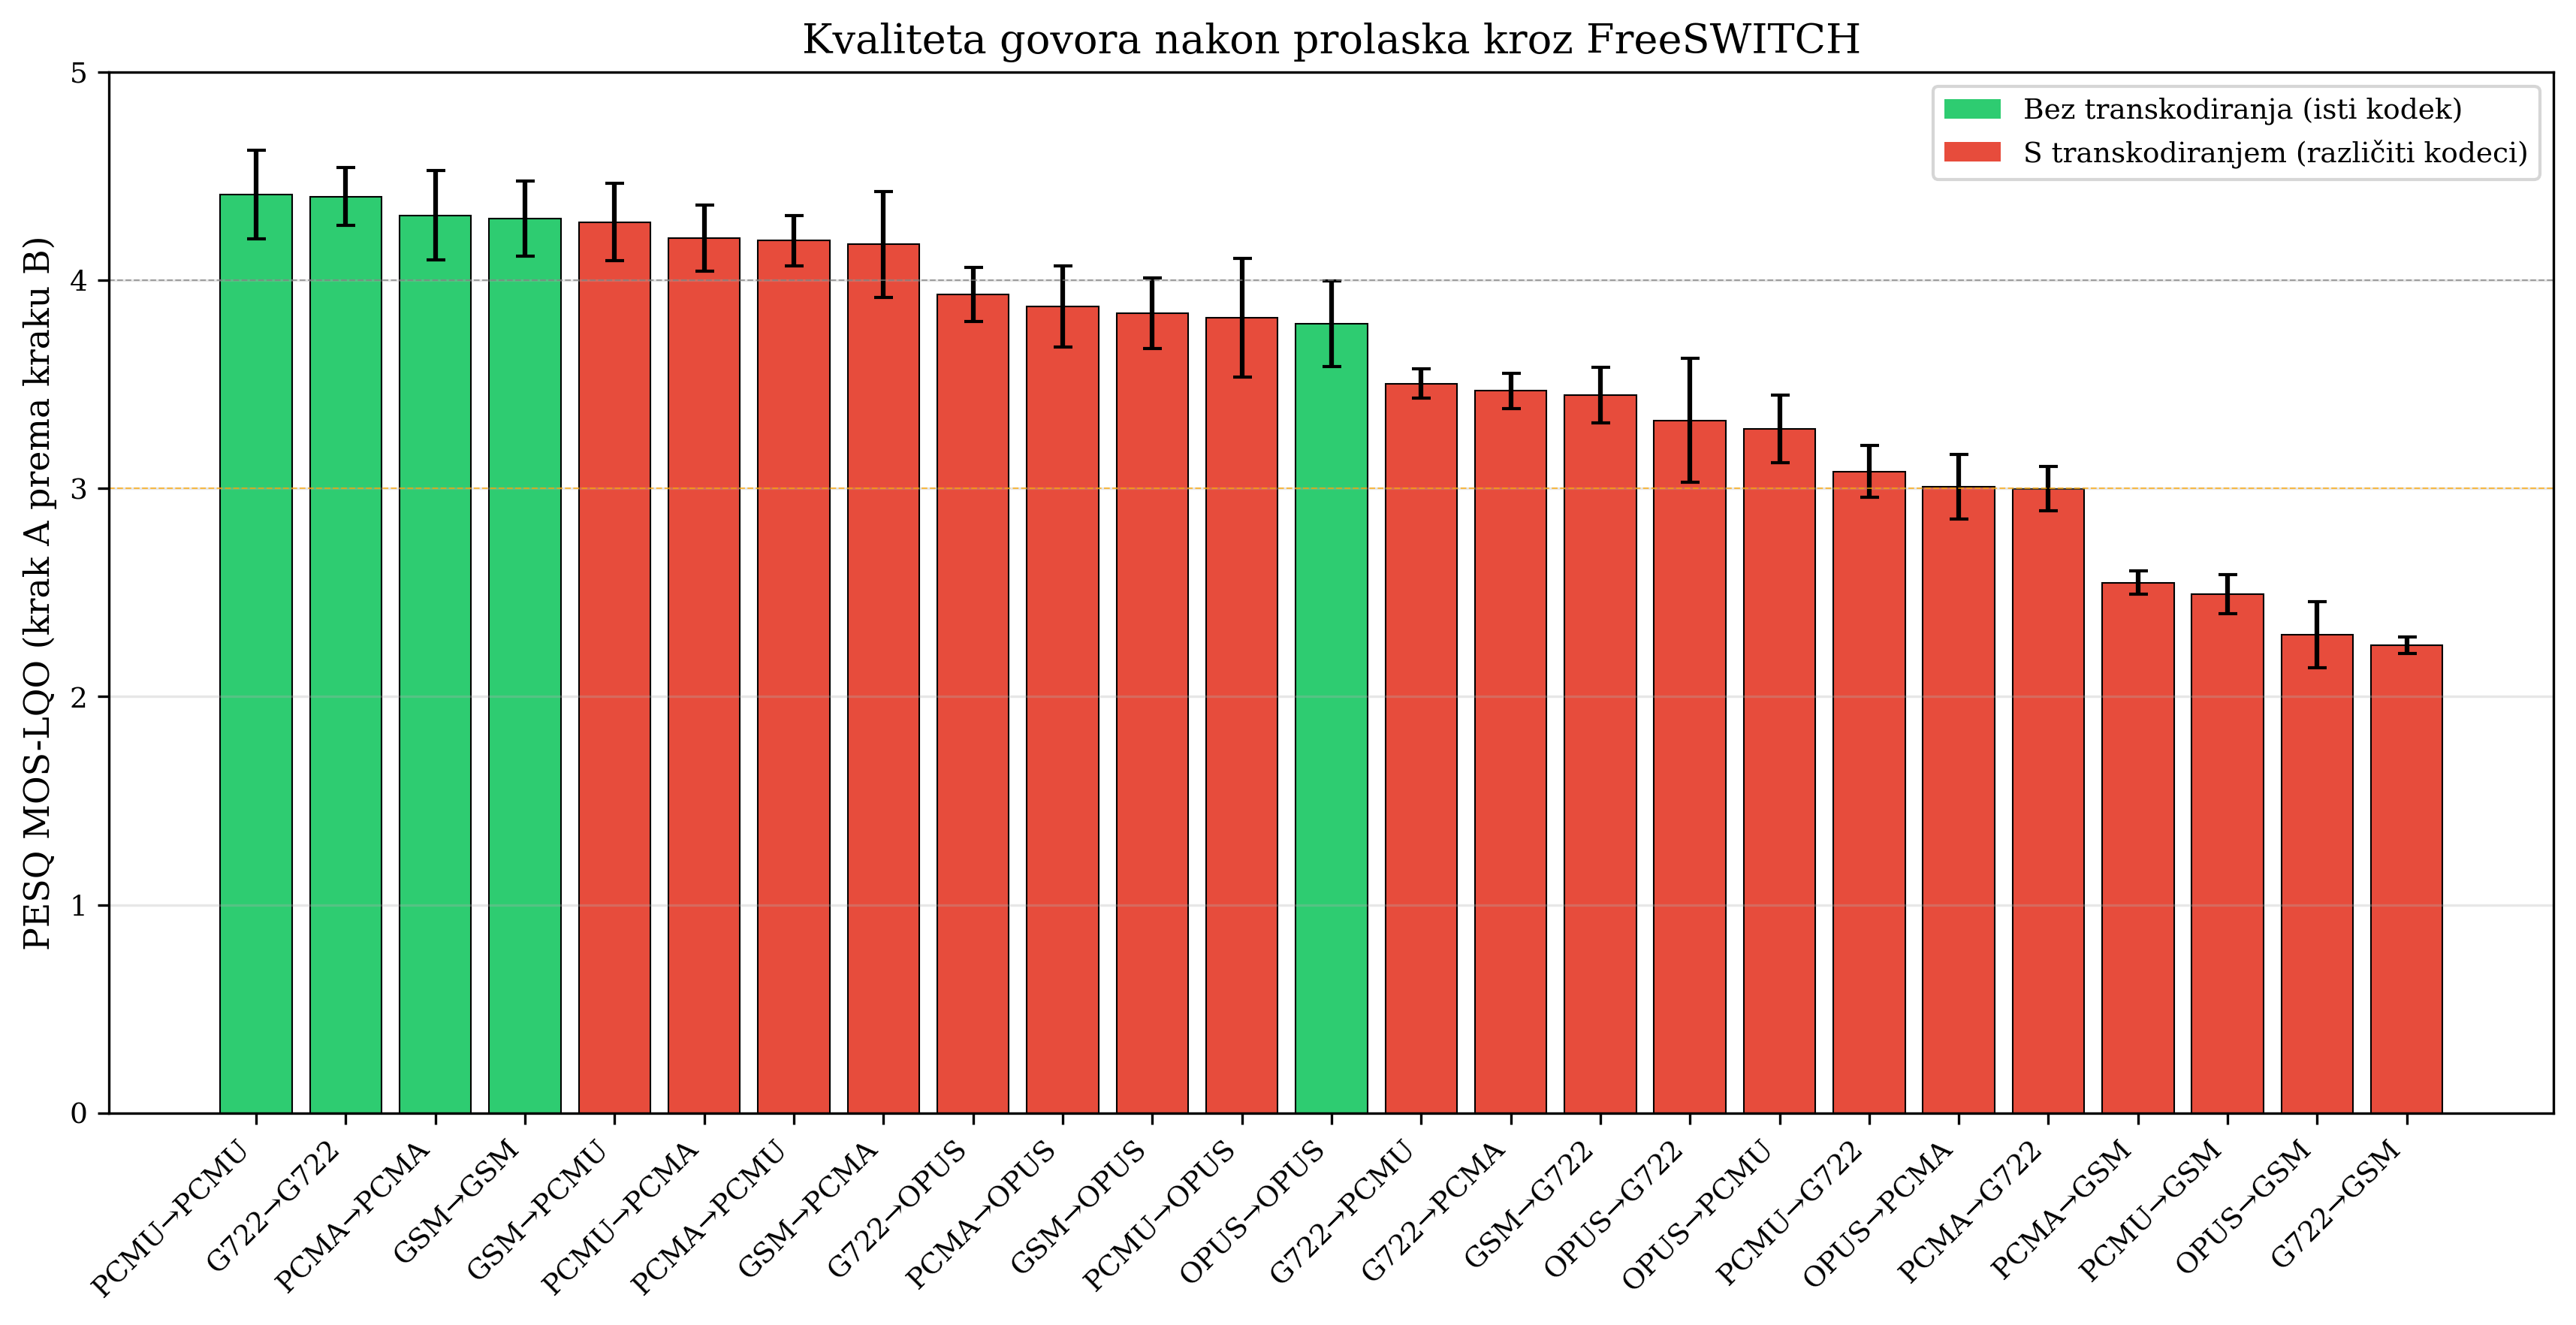
\includegraphics[width=0.95\textwidth]{pesq_mos_bars.png}
\caption{PESQ MOS-LQO za sve kombinacije; greške prikazuju uzoračku standardnu devijaciju deset ponavljanja}
\label{fig:pesq-bars}
\end{figure}

\begin{figure}[htbp]
\centering
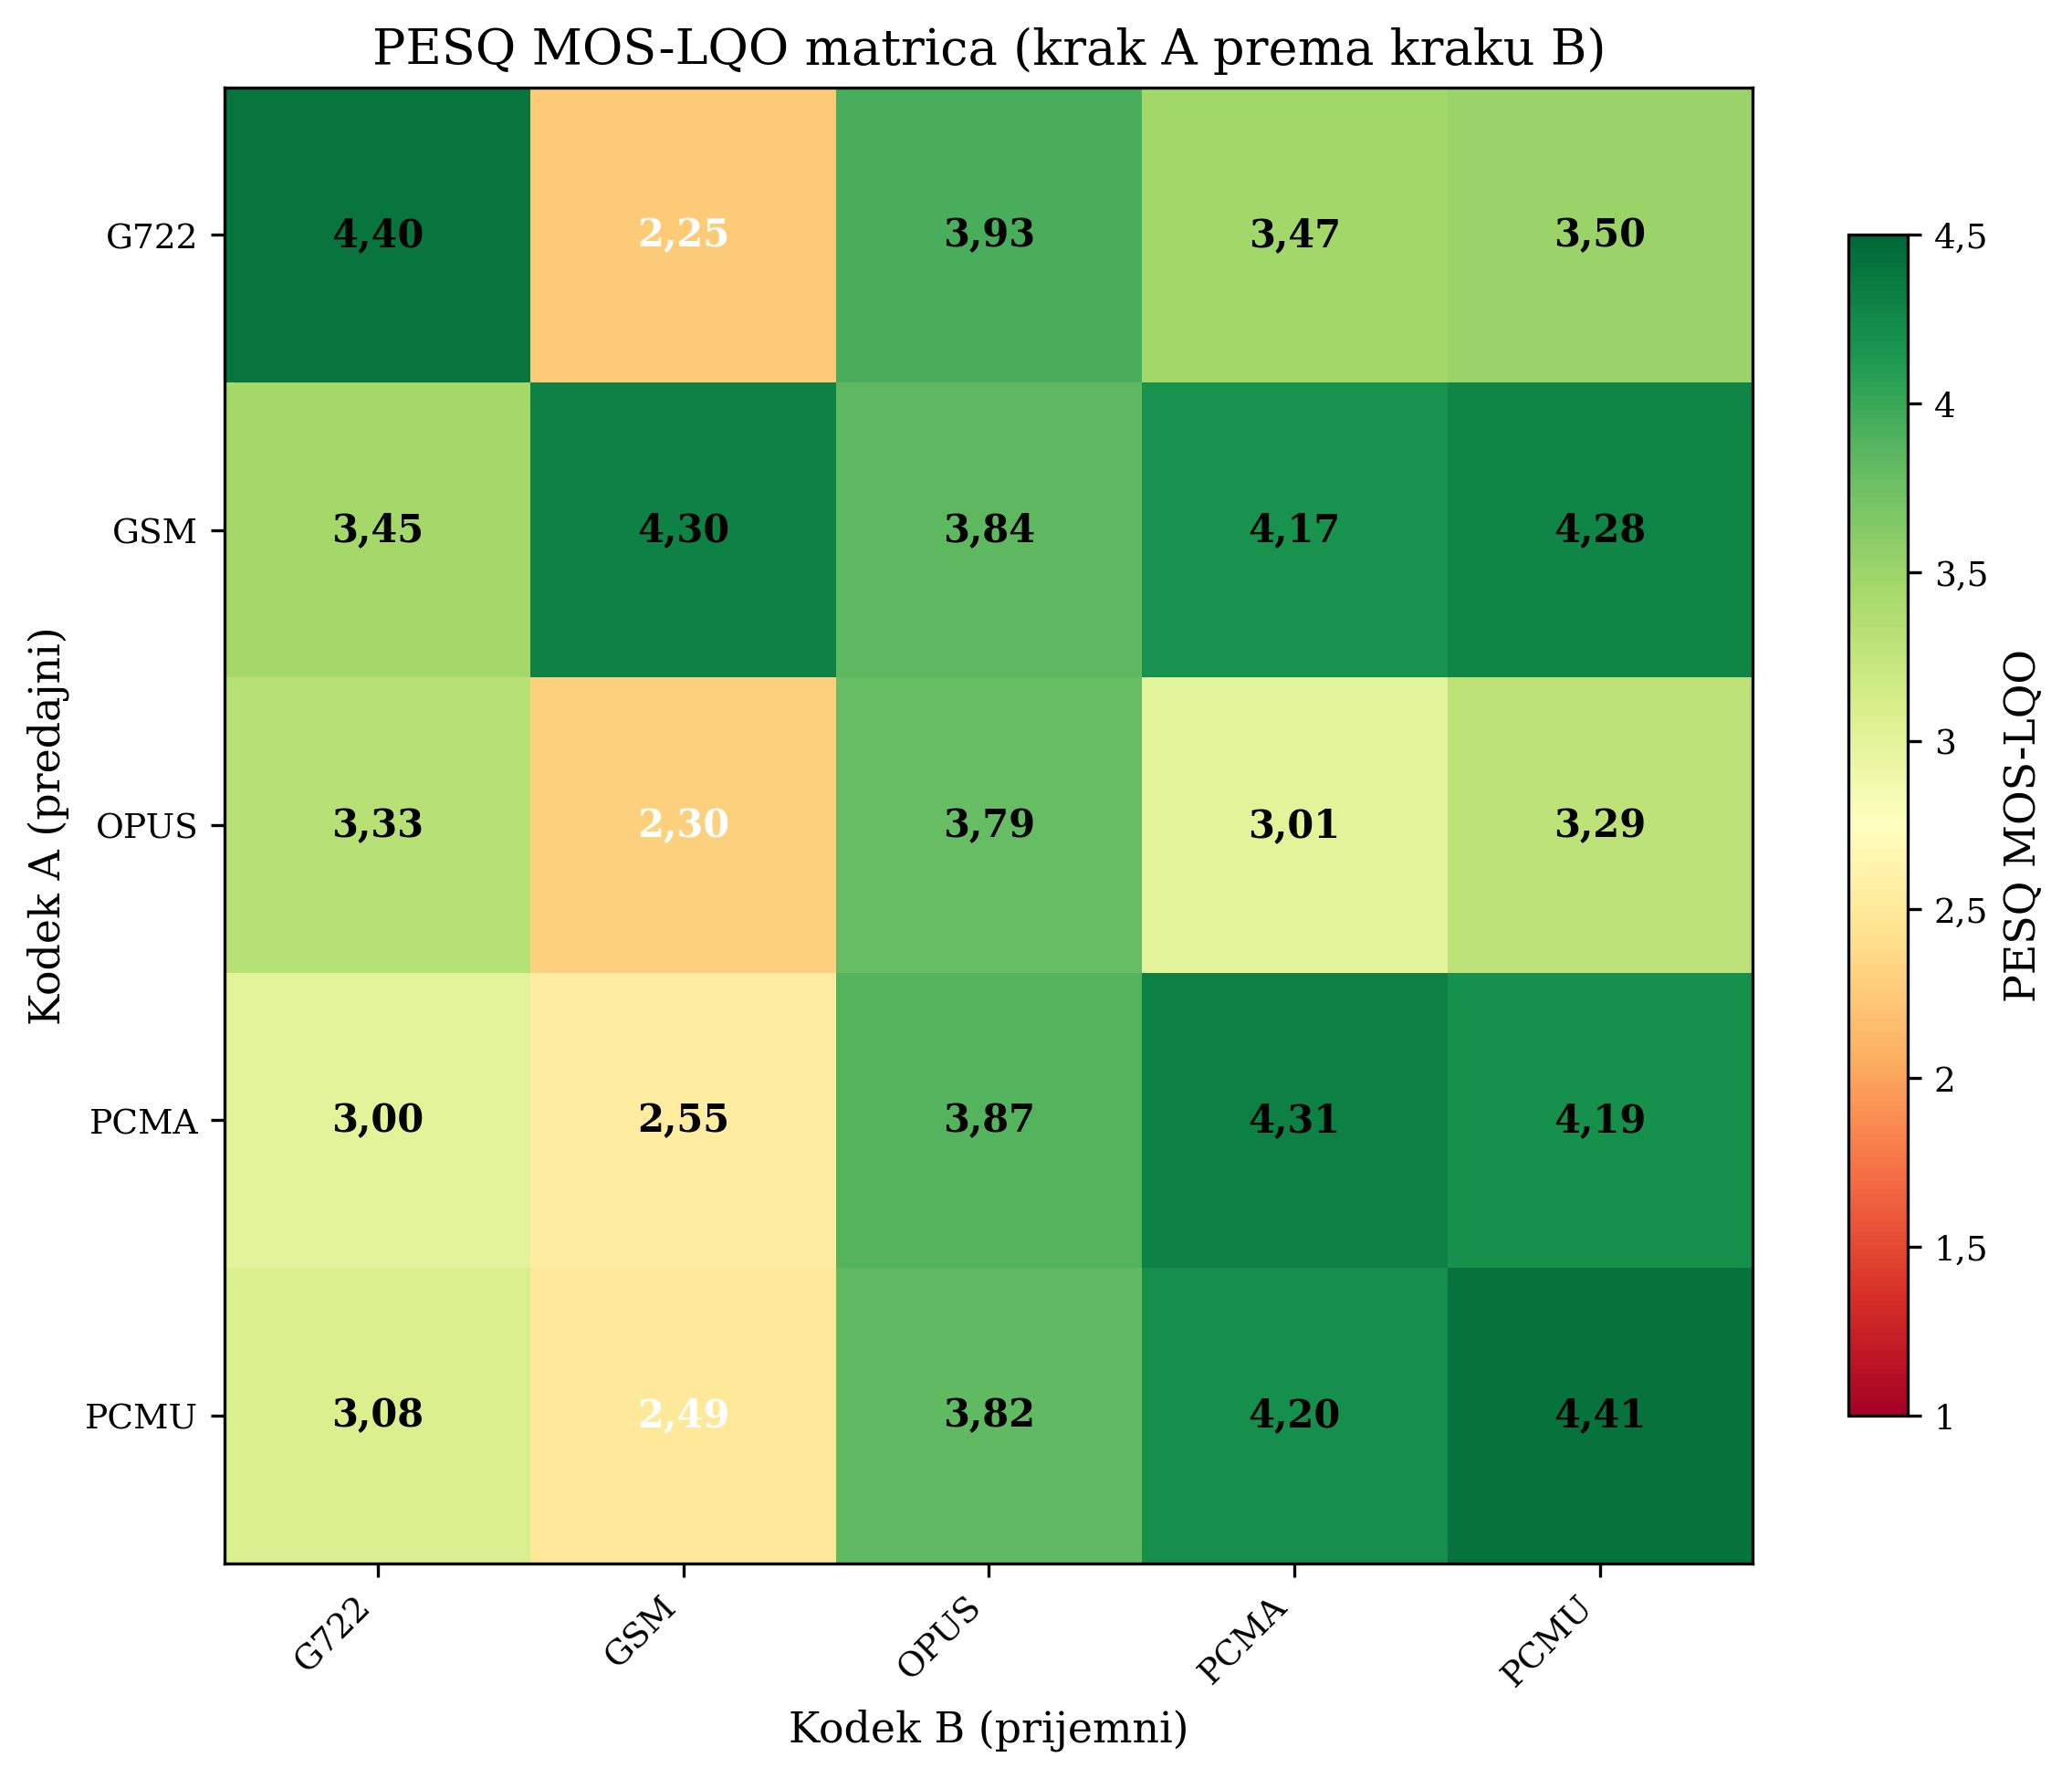
\includegraphics[width=0.85\textwidth]{codec_heatmap.png}
\caption{Puna matrica PESQ MOS-LQO rezultata}
\label{fig:heatmap}
\end{figure}

\begin{figure}[htbp]
\centering
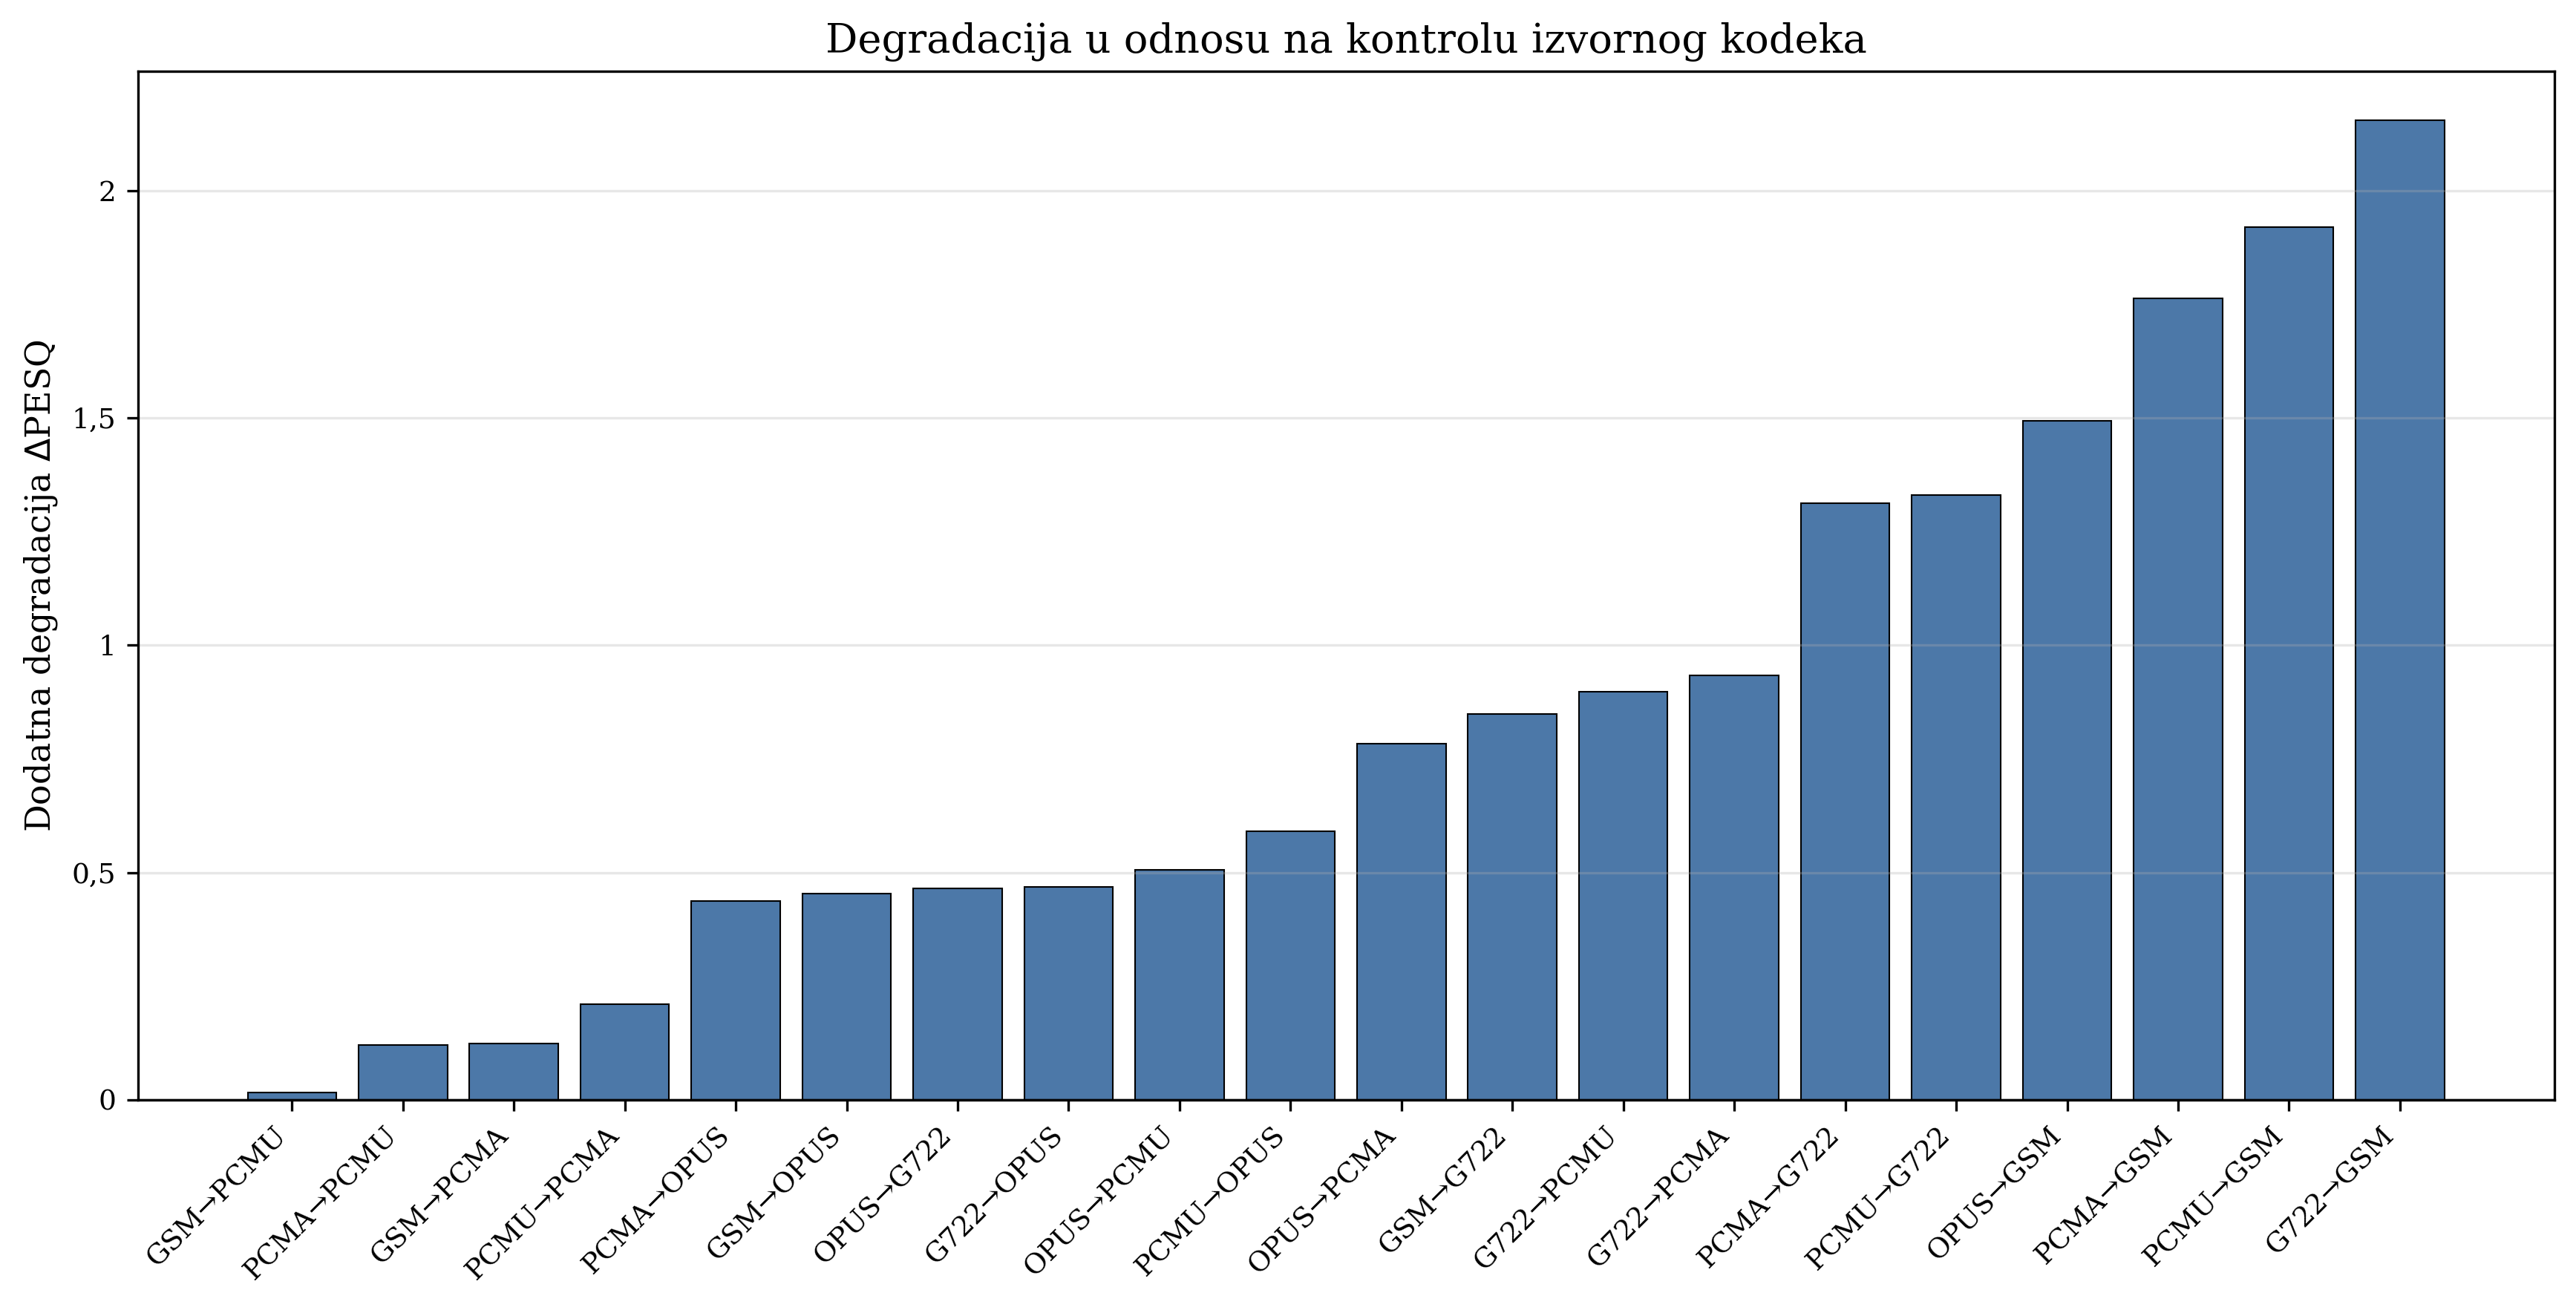
\includegraphics[width=0.95\textwidth]{pesq_degradation.png}
\caption{Dodatna degradacija u odnosu na kontrolu istog izvornog kodeka}
\label{fig:pesq-degradation}
\end{figure}

\FloatBarrier
\section{Utjecaj smjera konverzije}

Rezultati su usmjereni: $A\rightarrow B$ i $B\rightarrow A$ obuhvataju različit odredišni koder i, kod kodeka različitog opsega, različitu promjenu frekvencije uzorkovanja. Tabela~\ref{tab:directional-asymmetry} zato neposredno uspoređuje svih deset neuređenih parova.

% Automatski generisano; ne uređivati ručno.
\begin{table}[htbp]
\centering
\caption{Razlika rezultata između suprotnih smjerova transkodiranja}
\label{tab:directional-asymmetry}
\small
\begin{tabular}{|l|c|c|c|}
\hline
\textbf{Par kodeka} & \textbf{prvi$\rightarrow$drugi} & \textbf{drugi$\rightarrow$prvi} & \textbf{Apsolutna razlika} \\
\hline
PCMU/PCMA & 4,202 & 4,191 & 0,011 \\
PCMU/G.722 & 3,081 & 3,504 & 0,423 \\
PCMU/Opus & 3,821 & 3,286 & 0,535 \\
PCMU/GSM & 2,492 & 4,279 & 1,787 \\
PCMA/G.722 & 2,999 & 3,468 & 0,469 \\
PCMA/Opus & 3,874 & 3,009 & 0,865 \\
PCMA/GSM & 2,548 & 4,172 & 1,624 \\
G.722/Opus & 3,932 & 3,327 & 0,605 \\
G.722/GSM & 2,246 & 3,448 & 1,202 \\
Opus/GSM & 2,298 & 3,842 & 1,544 \\
\hline
\end{tabular}
\end{table}


Razlike između suprotnih smjerova potvrđuju da se rezultat jednog smjera ne smije preslikati na drugi. To je praktično važno pri definisanju prioriteta kodeka jer ista dva krajnja formata mogu dati različitu dodatnu degradaciju zavisno od toga koji se koristi na izlaznom kraku.

\section{Eksplorativna statistička provjera}

Primarni nalaz je deskriptivan jer matrica sadrži sve usmjerene parove pet odabranih kodeka. Kao dopunska provjera, dvadeset konfiguracijskih vrijednosti $\Delta_{A\rightarrow B}$ uspoređeno je s nulom. Dvostrani test daje $t=\DeltaT$ uz \DeltaDF{} stepeni slobode i $p=\DeltaP$. Prosječna dodatna degradacija iznosi \RazlikaPESQ{} MOS-LQO boda. Njen 95-postotni interval pouzdanosti kreće se od \RazlikaCIDonja{} do \RazlikaCIGornja{}, a korigirana Hedgesova mjera iznosi $g=\HedgesG$. Test opisuje razlike među odabranim konfiguracijama. Deset tehničkih ponavljanja ne predstavlja deset različitih govornika, pa se rezultat ne može proširiti na sve moguće kodeke i govornike.

\section{STOI i procesorsko opterećenje}

Prosječni STOI kontrolnih konfiguracija iznosi približno 0,996, dok kod konfiguracija s transkodiranjem ostaje visok. STOI se ovdje računa u odnosu na krak A, a promjene frekvencije uzorkovanja i različite osnovne vrijednosti kodeka utječu na grupni prosjek. Zato se koristi kao pomoćna provjera očuvanja razumljivosti, bez tvrdnje da transkodiranje može poboljšati izvorni govor.

Prosječno opterećenje FreeSWITCH kontejnera iznosi \PassthroughCPU{} bez transkodiranja i \TranscodeCPU{} s transkodiranjem, odnosno približno \OmjerCPU{} puta više. Najveće vrijednosti imaju konfiguracije koje kodiraju u Opus. Pošto mjerenje obuhvata cijeli kontejner, osnovno opterećenje i dio pripremnog intervala, rezultat je relativna usporedba na ispitnom računaru, a ne univerzalna cijena jednog poziva. Vrijednosti po konfiguraciji prikazane su na Slici~\ref{fig:cpu-bars}.

\begin{figure}[htbp]
\centering
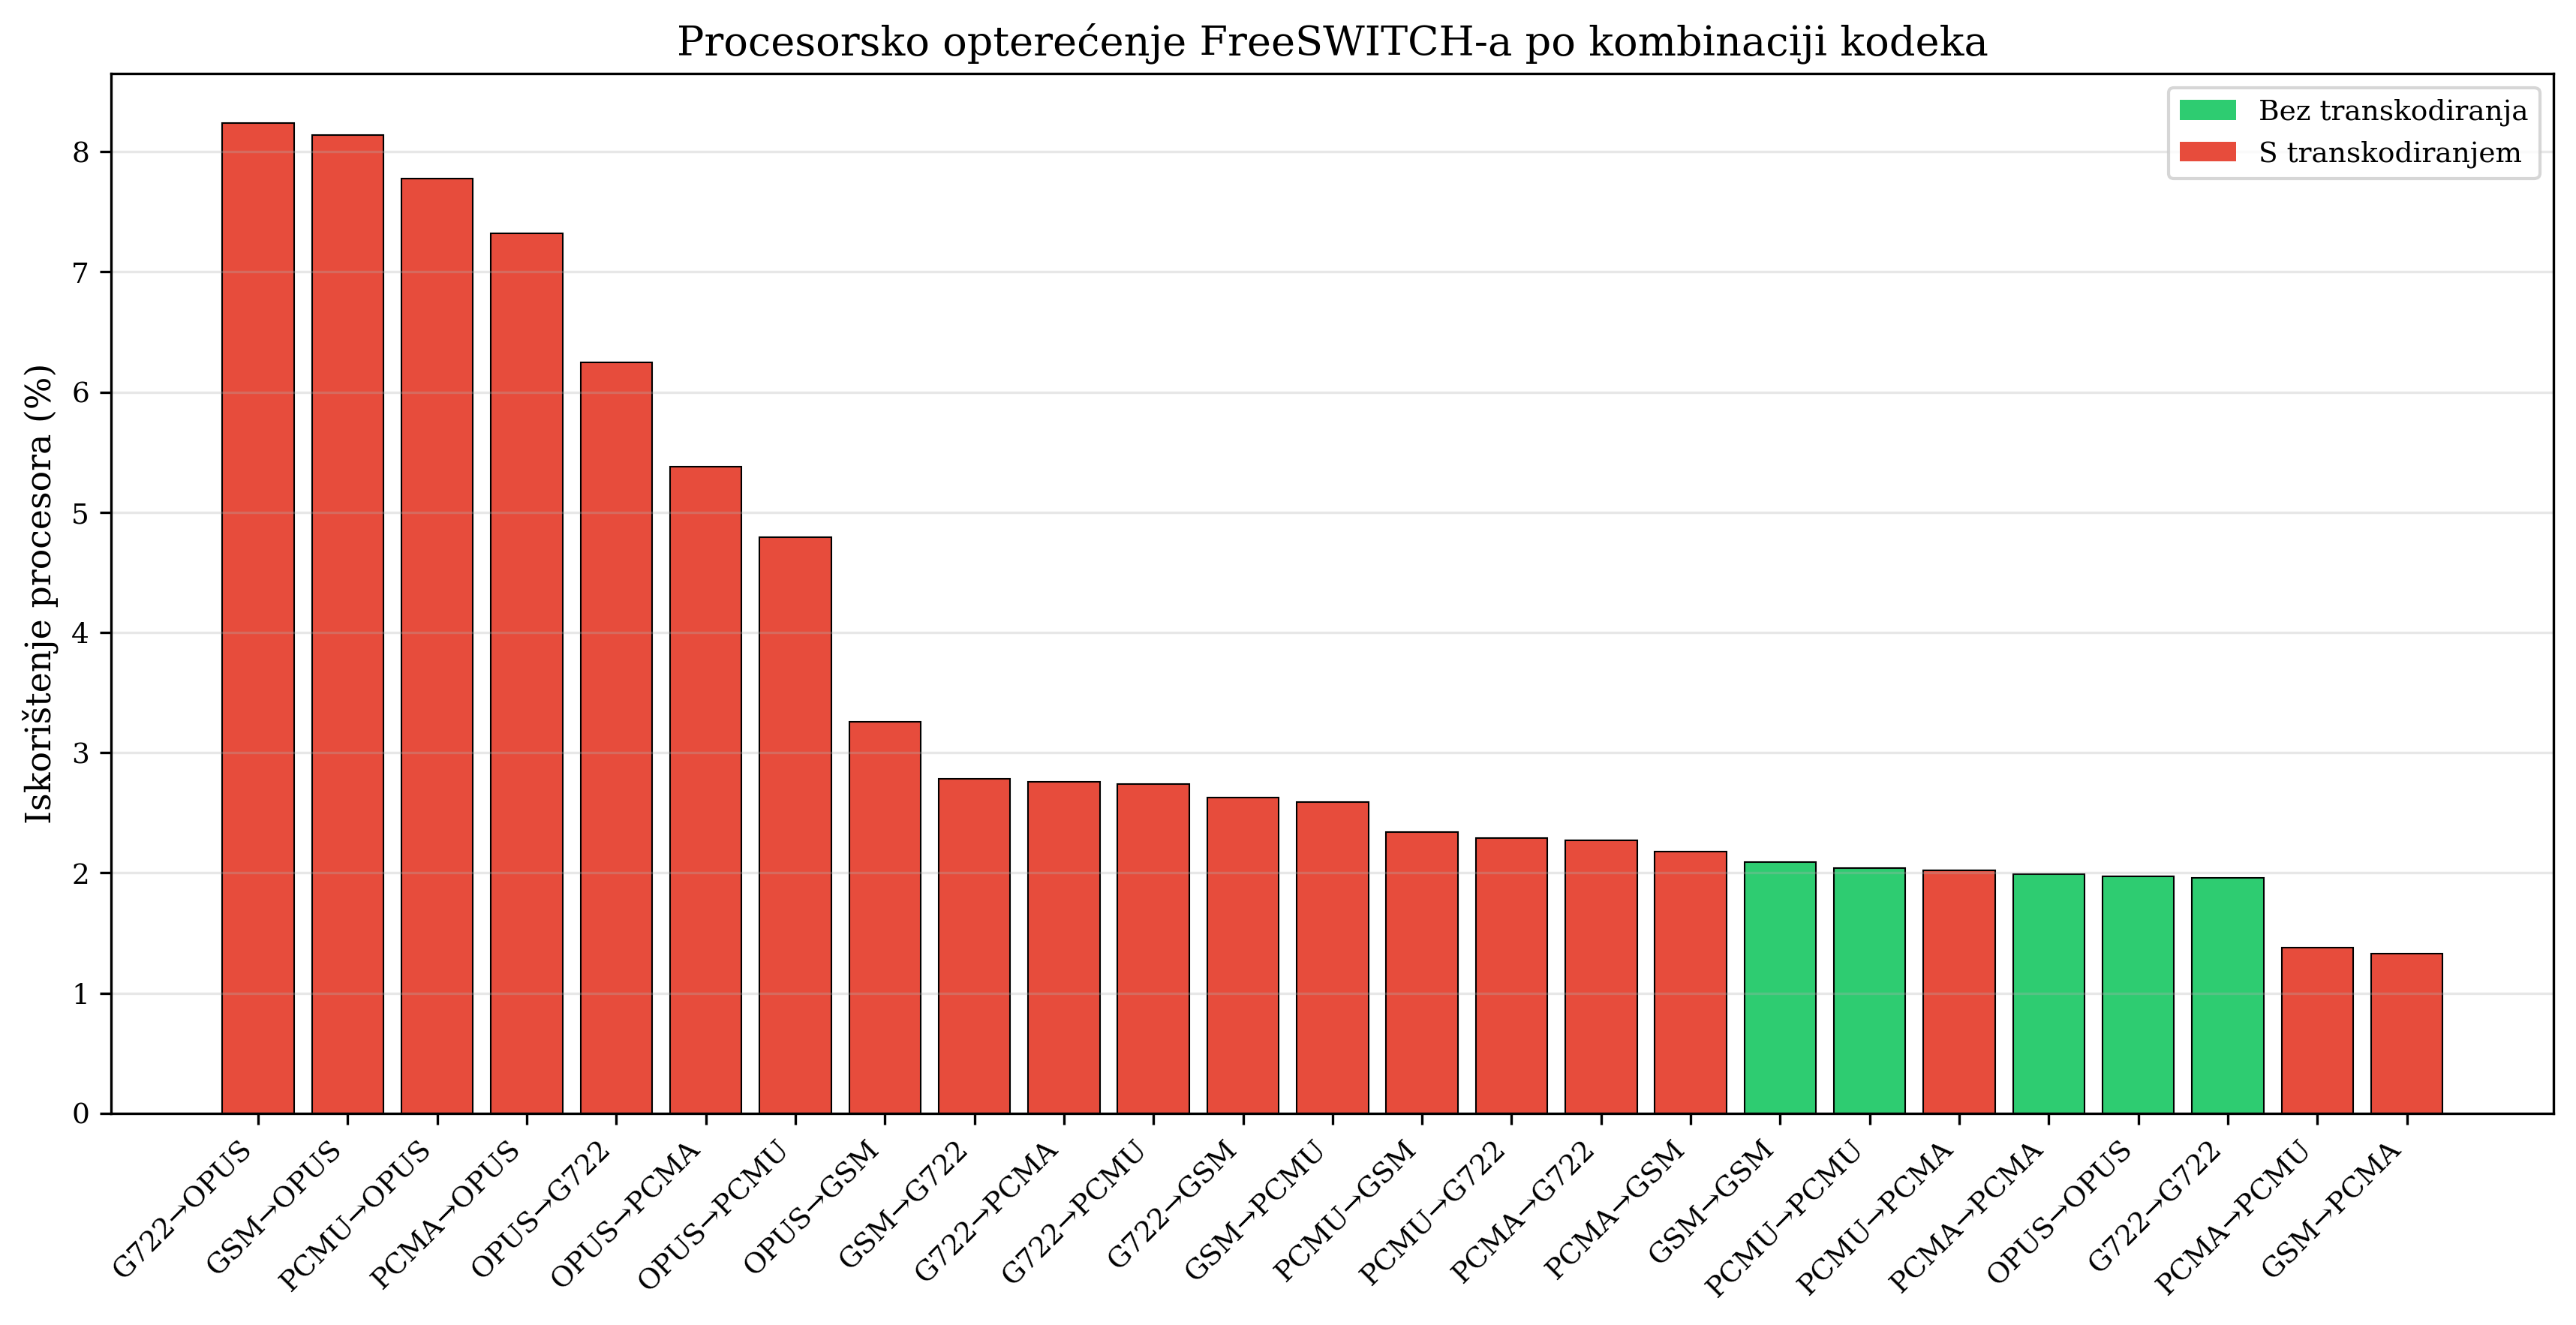
\includegraphics[width=0.95\textwidth]{cpu_usage_bars.png}
\caption{Prosječna potrošnja procesora FreeSWITCH kontejnera po konfiguraciji}
\label{fig:cpu-bars}
\end{figure}

\FloatBarrier
\section{Dopunska end-to-end analiza}
\label{sec:e2e-results}

Primarna analiza pokazuje koliko se B-leg razlikuje od signala koji je FreeSWITCH primio na A-legu. Dopunska analiza koristi originalni reproducirani WAV kao referencu i zato uključuje početno kodiranje kodekom A, obradu na serveru i završno kodiranje kodekom B. Za istih 250 poziva prosječni WB PESQ na 16 kHz iznosi 3,170 za pet kontrola bez transkodiranja i 2,608 za dvadeset transkodiranih konfiguracija. Odgovarajući prosjeci STOI su 0,983 i 0,932.

Na nivou pojedinačnih poziva WB PESQ je u rasponu 1,750--3,944, a STOI u rasponu 0,817--0,996. Raspon nije sam po sebi rang-lista kodeka: svaka konfiguracija uključuje ograničenje izvornog kodeka A, a vrijednost zavisi i od odredišnog kodera. Zbog toga se transkodirana putanja poredi s end-to-end kontrolom istog izvora. Prosjek tako definisane dodatne degradacije iznosi 0,563 PESQ boda.

% Izvor: results/end_to_end_original_vs_bleg_20260828/summary_by_configuration.csv
\begin{table}[htbp]
\centering
\caption{End-to-end rezultat prema izvornom kodeku na kraku A}
\label{tab:e2e-by-source}
\small
\begin{tabular}{|l|c|c|c|c|}
\hline
\textbf{Izvor A} & \textbf{Kontrola} & \textbf{Prosjek ostalih} & \textbf{Prosječni $\Delta$} & \textbf{STOI ostalih} \\
\hline
PCMU  & 3,688 & 2,982 & 0,706 & 0,9625 \\
PCMA  & 3,708 & 3,013 & 0,695 & 0,9535 \\
G.722 & 2,868 & 2,435 & 0,433 & 0,9685 \\
GSM   & 2,294 & 2,229 & 0,065 & 0,9213 \\
Opus  & 3,294 & 2,381 & 0,913 & 0,8555 \\
\hline
\end{tabular}
\end{table}


Tabela~\ref{tab:e2e-by-source} pokazuje zašto je izbor reference važan. GSM kontrola već ima WB PESQ 2,294 prema originalu. Ostale putanje koje počinju GSM-om prosječno daju 2,229, pa je dodatna razlika samo 0,065. Mali dodatni gubitak ne znači visok apsolutni kvalitet, nego da kasniji koder uglavnom čuva signal koji je već ograničen GSM kodiranjem. Suprotno tome, Opus kontrola iznosi 3,294, a prosjek njegovih transkodiranih izlaza 2,381, jer odredišni uskopojasni kodeci odbacuju dio informacije prisutan na ulazu. Odnosi svih izvornih i odredišnih kodeka prikazani su na Slici~\ref{fig:e2e-heatmap}.

\begin{figure}[htbp]
\centering
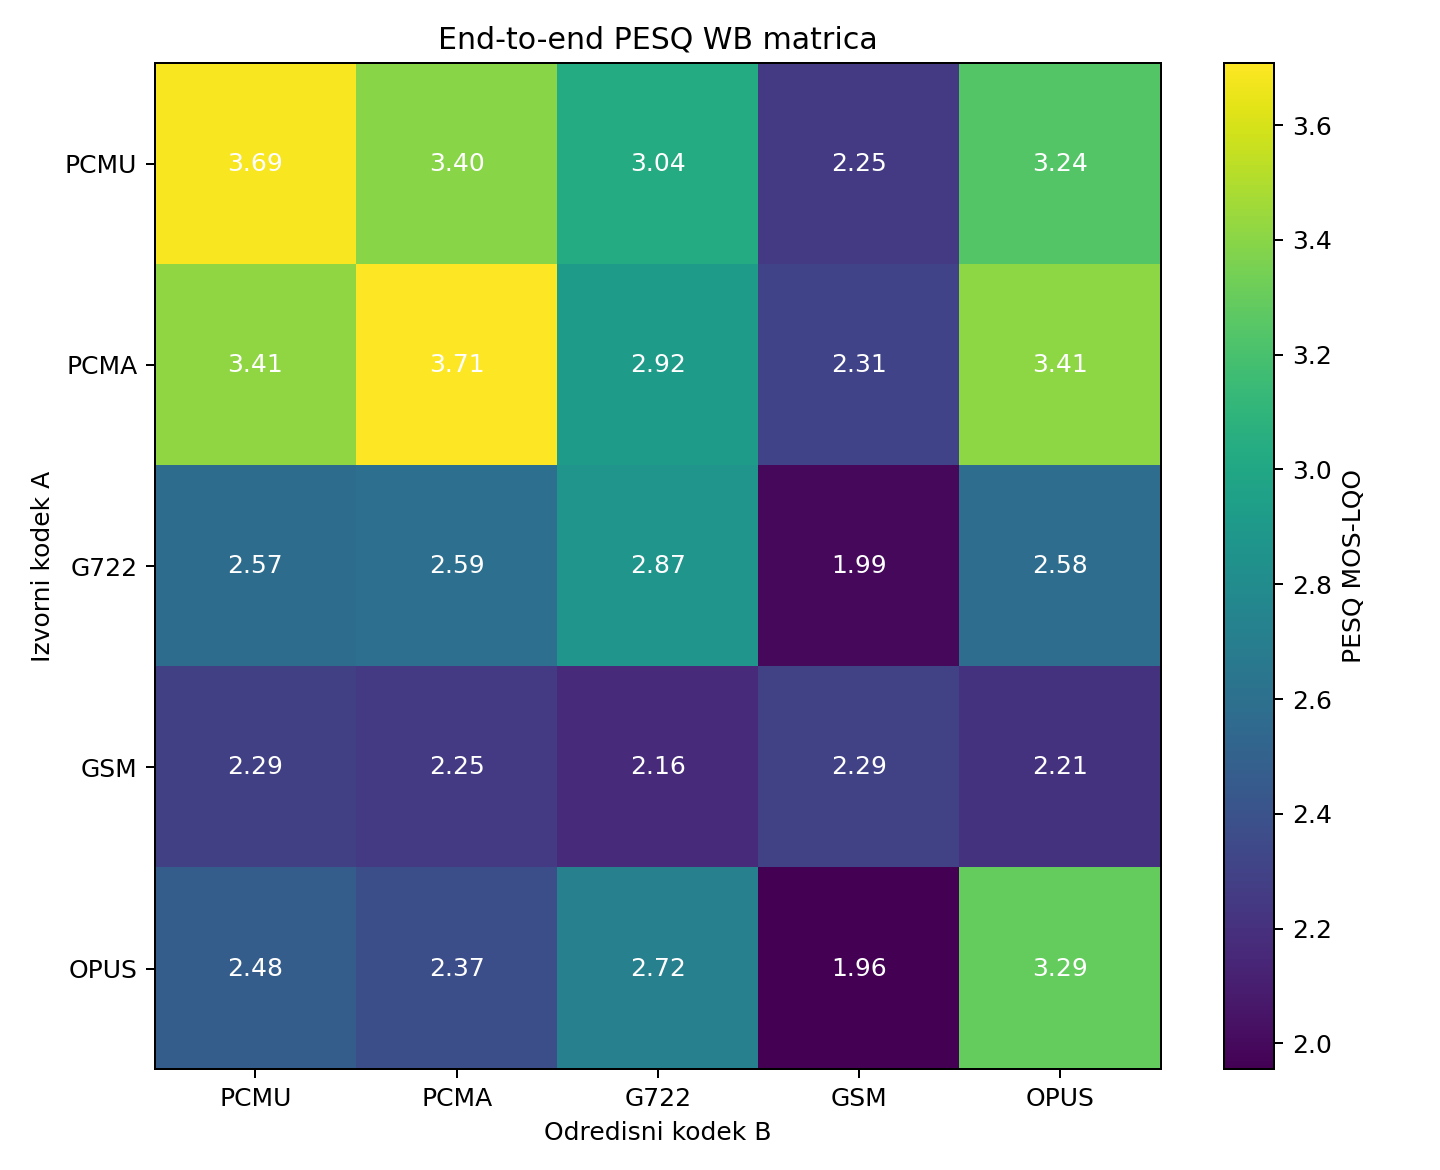
\includegraphics[width=0.82\textwidth]{../results/end_to_end_original_vs_bleg_20260828/charts/pesq_wb_16k_heatmap.png}
\caption{End-to-end WB PESQ matrica: originalni WAV prema izlaznom B-legu}
\label{fig:e2e-heatmap}
\end{figure}

Najviše apsolutne WB PESQ vrijednosti među transkodiranim konfiguracijama imaju sljedeće putanje:

\begin{itemize}
    \item PCMA$\rightarrow$PCMU: 3,414;
    \item PCMA$\rightarrow$Opus: 3,408;
    \item PCMU$\rightarrow$PCMA: 3,396.
\end{itemize}

Njihov izvor nije prethodno prošao kroz snažno kompresijski govorni model, a odredište ne uvodi uskopojasno kodiranje niske brzine poput GSM-a. Najniže vrijednosti imaju Opus$\rightarrow$GSM (1,955) i G.722$\rightarrow$GSM (1,993), gdje se širokopojasni izvor svodi na uskopojasni GSM format.

Spektralna analiza dodatno pokazuje šta se događa u smjeru Opus$\rightarrow$GSM. Posmatrano kroz svih deset ponavljanja, prosječni udio energije u opsegu 3,4--7 kHz smanjen je sa 2,84\% u izvornom signalu na 0,08\% u krajnjem B-legu. Frekvencija ispod koje se nalazi 95\% spektralne energije pomjerena je sa 2763 Hz na 1646 Hz. Na Slici~\ref{fig:opus-gsm-spectrum} prikazana je reprezentativna peta iteracija, čiji je PESQ najbliži prosjeku konfiguracije. Vremenski oblik zadržava osnovnu strukturu govora, dok spektrogram i prosječna raspodjela spektralne snage jasno pokazuju potiskivanje viših frekvencija nakon kodiranja u GSM.

\begin{figure}[htbp]
\centering
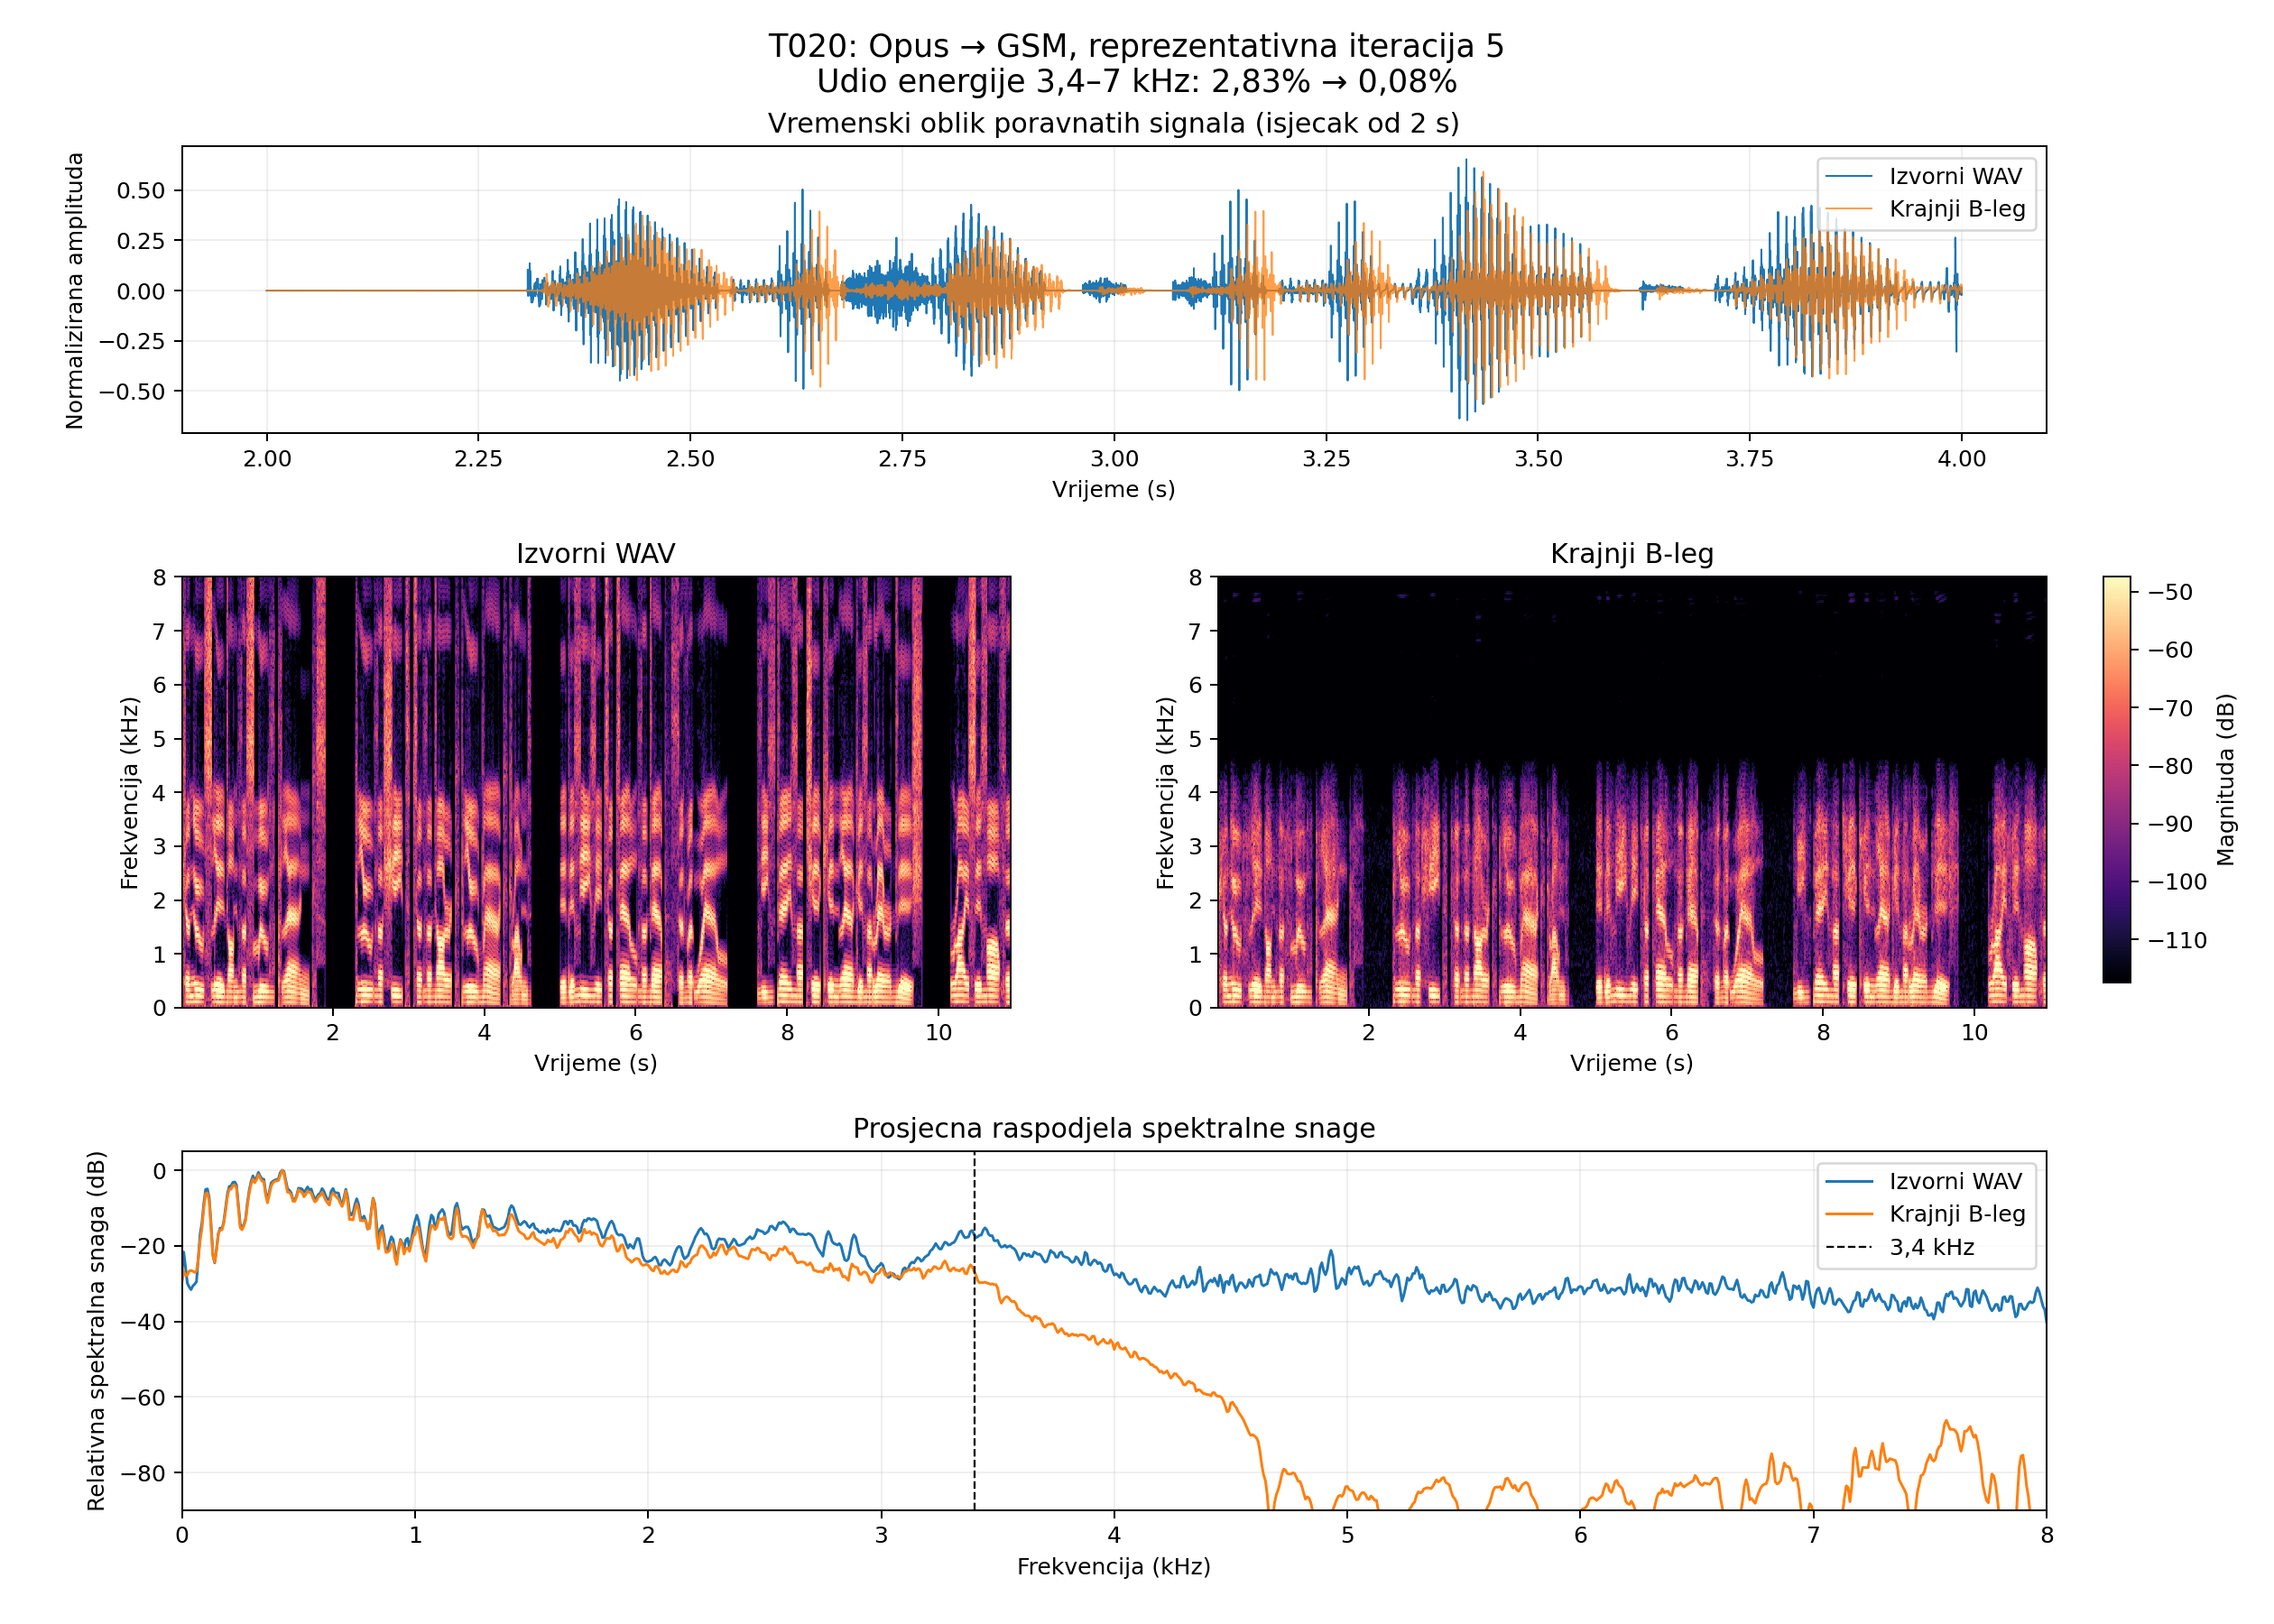
\includegraphics[width=0.98\textwidth]{opus_to_gsm_signal_comparison.png}
\caption{Poređenje izvornog signala i krajnjeg B-lega za konfiguraciju Opus$\rightarrow$GSM}
\label{fig:opus-gsm-spectrum}
\end{figure}

Isti obrazac vidi se u dodatnoj degradaciji prema kontroli izvornog kodeka. Najveće vrijednosti imaju PCMU$\rightarrow$GSM (1,434), PCMA$\rightarrow$GSM (1,398) i Opus$\rightarrow$GSM (1,339). Najmanje su GSM$\rightarrow$PCMU (0,006), GSM$\rightarrow$PCMA (0,039) i GSM$\rightarrow$Opus (0,082). U prvom skupu završni GSM koder odbacuje znatan dio preostale informacije; u drugom skupu odredišni kodek malo mijenja već GSM-ograničeni signal.

Posebno ilustrativna je konfiguracija GSM$\rightarrow$PCMA. A-leg$\rightarrow$B-leg PESQ iznosi 4,172, što pokazuje da je FreeSWITCH vrlo malo promijenio ulazni GSM signal. End-to-end WB PESQ ipak iznosi 2,255 jer je najveći dio razlike prema originalu nastao prije ulaska u poslužitelj. Dodatna end-to-end degradacija u odnosu na GSM kontrolu iznosi samo 0,039 boda. Bez obje referentne tačke rezultat 4,172 mogao bi se pogrešno protumačiti kao visok konačni kvalitet. Poređenje svih konfiguracija prikazano je na Slici~\ref{fig:e2e-bars}.

\begin{figure}[htbp]
\centering
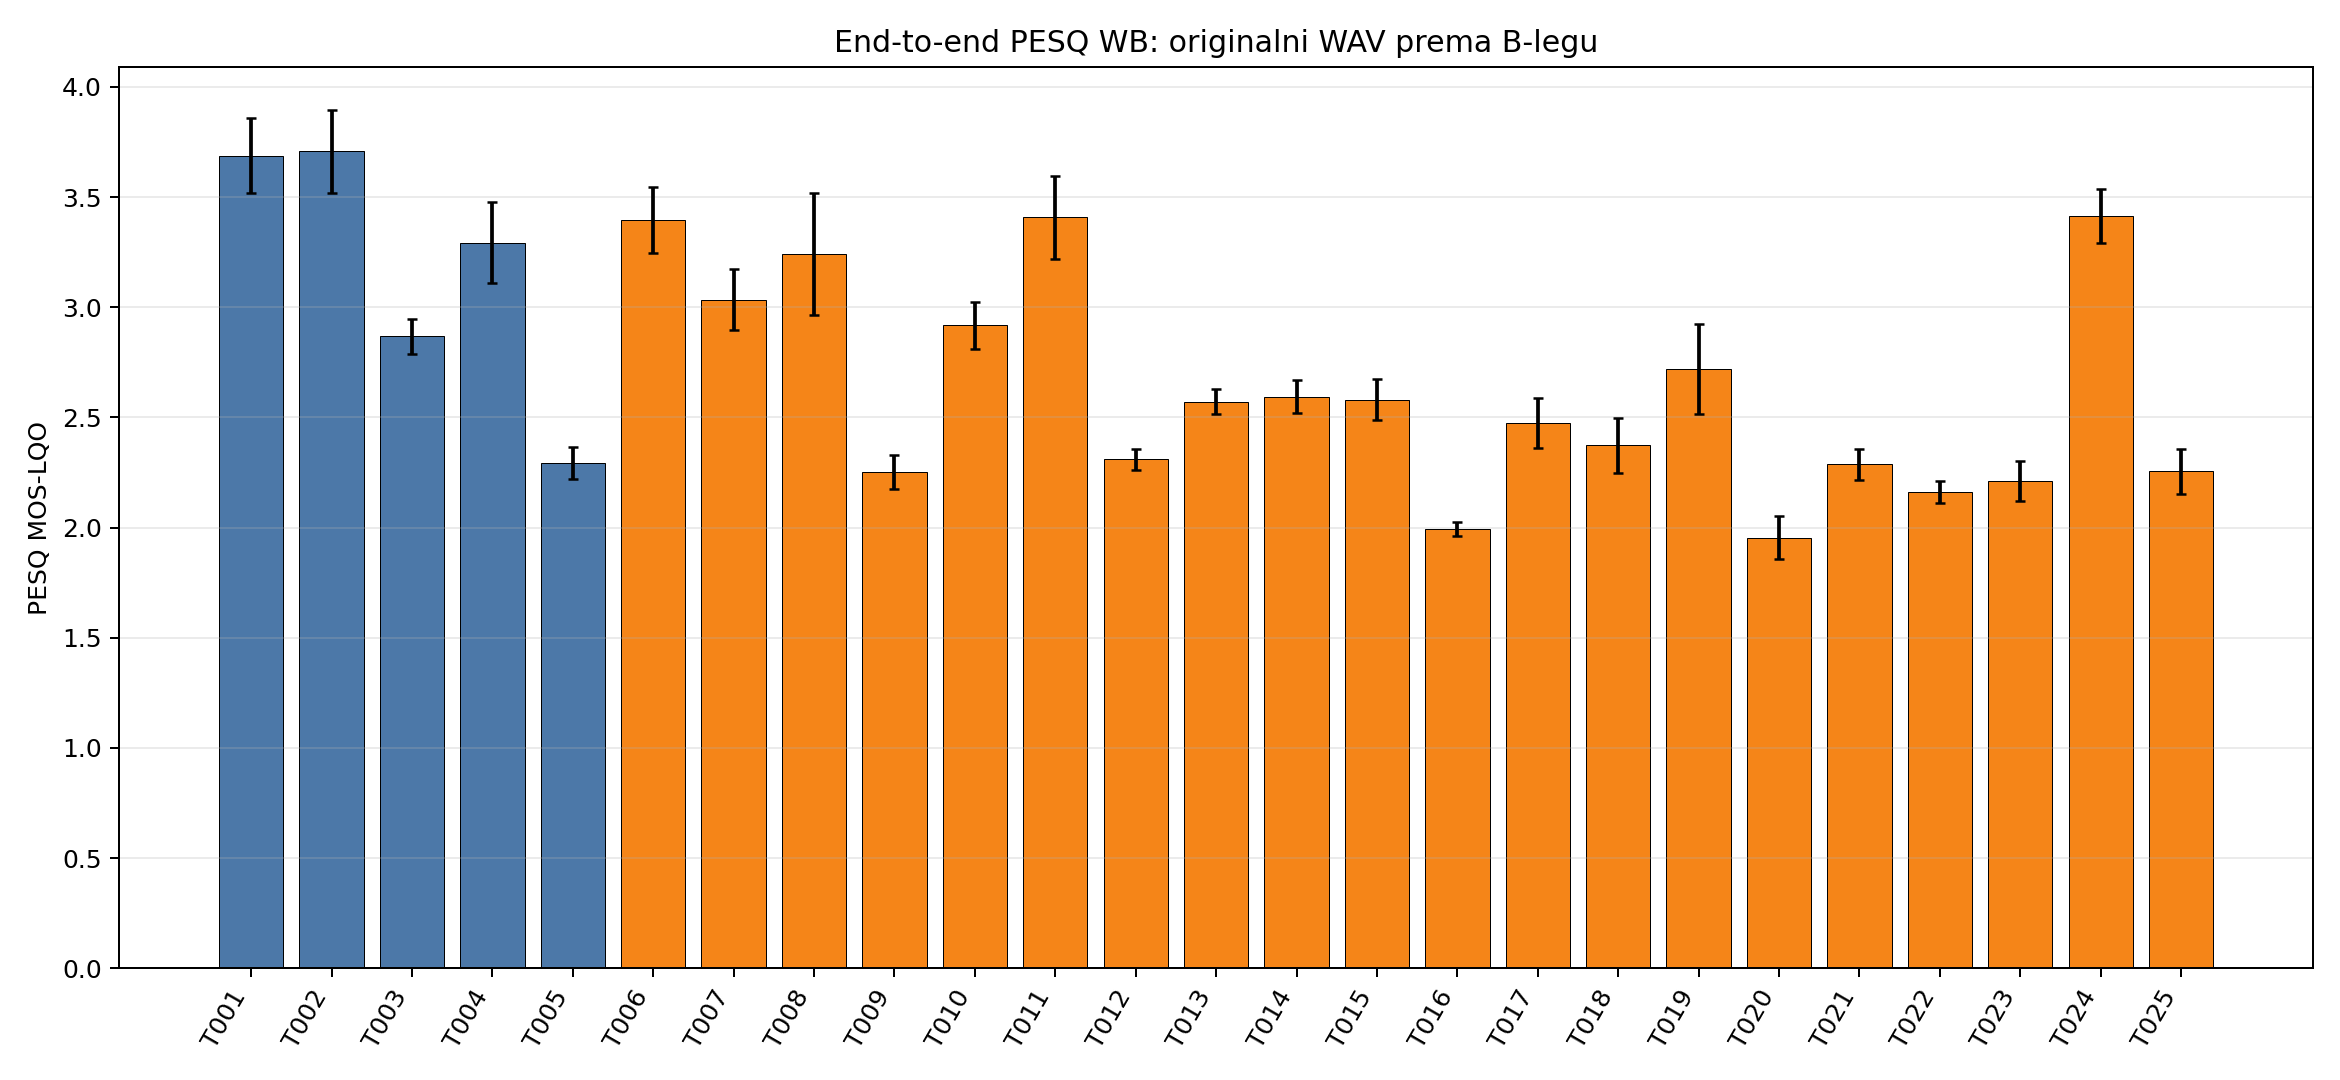
\includegraphics[width=0.95\textwidth]{../results/end_to_end_original_vs_bleg_20260828/charts/pesq_wb_16k_bars.png}
\caption{End-to-end WB PESQ po konfiguraciji; greške prikazuju standardnu devijaciju deset ponavljanja}
\label{fig:e2e-bars}
\end{figure}

Pored zajedničkog WB postupka, izračunat je PESQ u režimu izvornog opsega: NB na 8 kHz za PCMU, PCMA i GSM izvore, a WB na 16 kHz za G.722 i Opus. Taj prikaz je prikladniji za uskopojasne izvore, ali NB i WB vrijednosti ne treba objedinjavati u jednu rang-listu. Zaključci o tome koje putanje dodaju najmanje ili najviše degradacije ostaju kvalitativno usklađeni s fizičkim ograničenjima kodeka.

End-to-end STOI ostaje visok kod većine konfiguracija, što znači da je struktura važna za razumljivost uglavnom očuvana i kada PESQ bilježi perceptivnu degradaciju. Varijabilnost je izraženija u putanjama s Opusom, naročito kada je Opus izvor. Ovaj dio rezultata treba tumačiti uz ograničenje rekonstrukcije RTP Opus okvira u Ogg wrapper. Zbog toga PESQ i STOI predstavljaju dopunske, a ne međusobno zamjenjive pokazatelje.

Tehničke provjere uspješno su završene za svih 250 zapisa. Svaka konfiguracija ima deset rezultata, a svih 250 PCAP zapisa je jedinstveno. RTP vremenske oznake imaju pravilne cjelobrojne skokove. Sva poravnanja ostala su unutar zadanog vremenskog raspona. Time je dopunska analiza dovoljno konzistentna za usporedbu s primarnim nalazima, uz navedena ograničenja reference i Opus rekonstrukcije.

\section{Praktične implikacije}

Rezultati podržavaju korištenje zajedničkog kodeka na oba kraja kada je to moguće. Ako je transkodiranje neizbježno, politiku kodeka treba zasnivati na konkretnom smjeru, prihvatljivoj degradaciji, raspoloživoj propusnosti i procesorskom kapacitetu. U ovom okruženju kodiranje u Opus daje povoljan odnos očuvanja ulaznog signala i propusnosti u primarnoj analizi, ali uz najveće CPU opterećenje. End-to-end rezultati dodatno pokazuju da prelazak u širokopojasni format ne može vratiti sadržaj izgubljen u prethodnom uskopojasnom kodeku. Kodiranje u GSM zato treba ograničiti na slučajeve u kojima kompatibilnost ili ušteda propusnosti opravdavaju izmjerenu degradaciju.

Politika prioriteta u SDP ponudi treba uzeti u obzir oba kanala. Ako krajnji uređaji imaju zajednički prihvatljiv kodek, njegovo zadržavanje uklanja jednu fazu dekodiranja i ponovnog kodiranja. Direktna konverzija PCMU$\leftrightarrow$PCMA u ovom skupu ima relativno malu degradaciju jer ostaje na istoj frekvenciji uzorkovanja i koristi srodne PCM predstavnike. Ipak, rezultat nije potpuno identičan prolazu zbog različitih kvantizacijskih nivoa. Putanje prema GSM-u pokazuju suprotan slučaj: smanjena propusnost plaća se najvećim gubitkom kvaliteta, posebno kada je ulaz širokopojasan.

Za nadzor produkcijskog sistema korisno je odvojeno prikazivati dvije vrste pokazatelja. A-leg$\rightarrow$B-leg mjera pomaže otkriti neuobičajenu degradaciju u medijskom serveru, dok mjera original$\rightarrow$B-leg pokazuje šta na kraju ostaje od polaznog signala. Bez prve se uzrok lošeg rezultata teško lokalizuje, a bez druge dobar rezultat nakon već degradiranog izvora može izgledati bolje nego što ga korisnik čuje. Praktični nadzor zato treba povezati kodeke oba kraka, mrežne pokazatelje i procesorsko opterećenje sa jasno označenom referentnom tačkom kvaliteta.

CPU rezultati ne određuju kapacitet poslužitelja, ali pokazuju koje putanje treba posebno testirati pri dimenzioniranju i skaliranju. Veći broj istovremenih Opus kodera može postati ograničenje prije mrežne propusnosti, dok G.711 troši više mrežnog kapaciteta uz jednostavniju obradu. Konačna politika zato nije samo rangiranje PESQ vrijednosti: ona je izbor kompromisa između očuvanosti govora, dostupne propusnosti, broja istovremenih poziva i skupa kodeka koje podržavaju povezane mreže.
